\chapter{Resultados}

A continuación presentamos los resultados de entrenamiento para los diferentes modelos
y su desempeño en los sets de datos, para luego exhibir algoritmos de agregación en el
modelo federado.

Las siguientes figuras muestran las detecciones realizadas por el modelo fundacional (YOLO) en cada uno de los sets de datos, donde se evidencia una buena capacidad de detección de artefactos. 

\begin{figure}[H]
  \centering
  \vspace{0.5cm}
  \begin{subfigure}[b]{0.48\textwidth}
    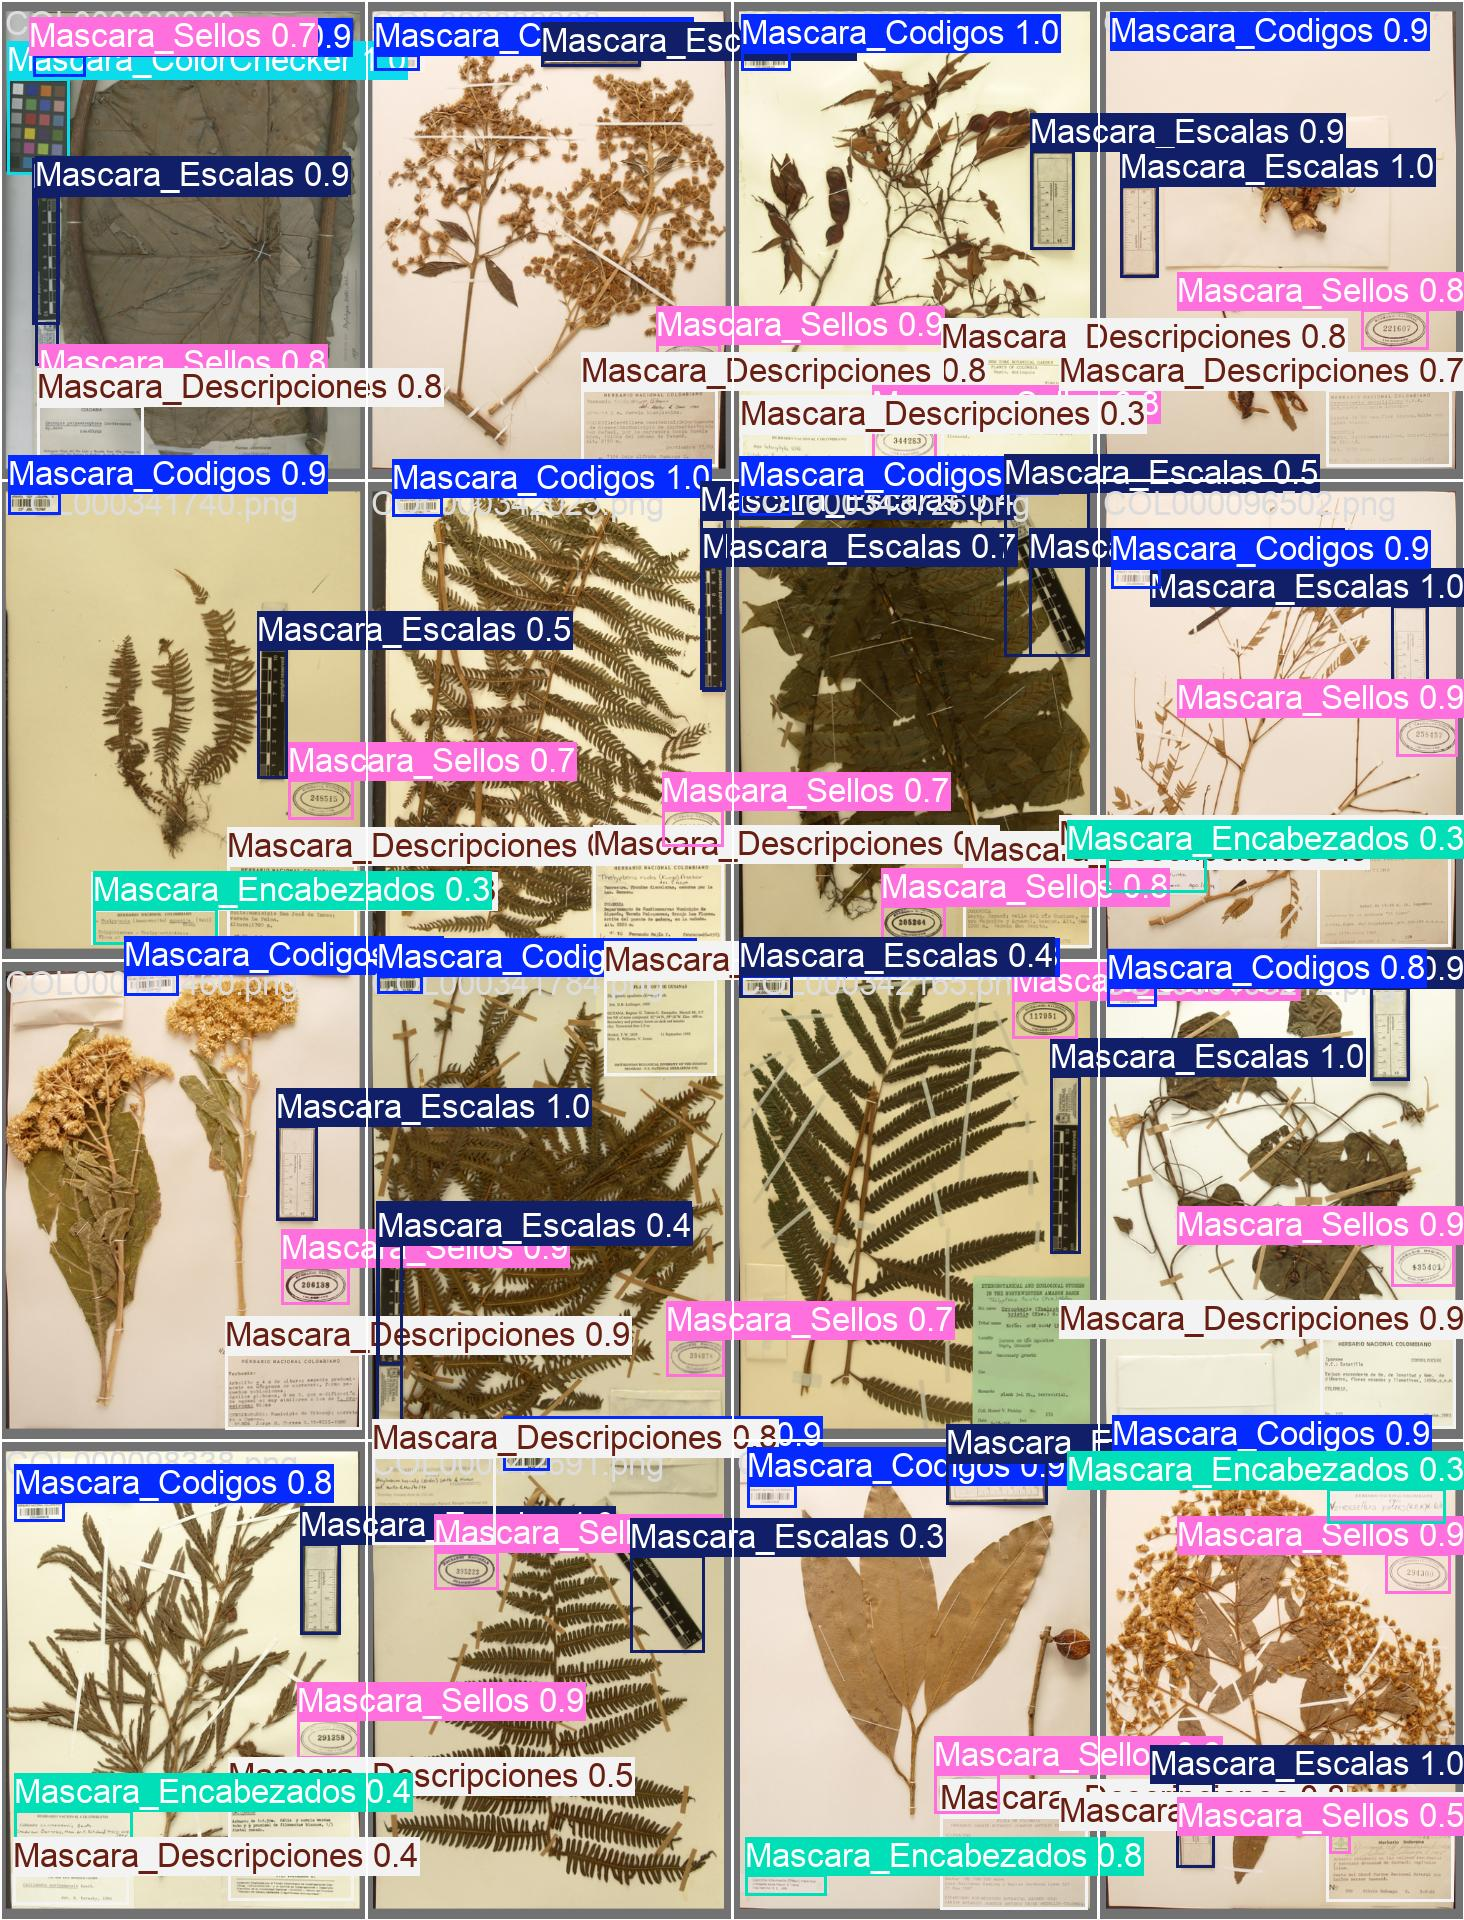
\includegraphics[width=\textwidth]{00Figuras/val_batch0_predClientUn.jpg}
    \caption{Performance de modelo YOLO con datos UN}
    \label{fig:image3}
  \end{subfigure}
  \hfill
  \begin{subfigure}[b]{0.48\textwidth}
    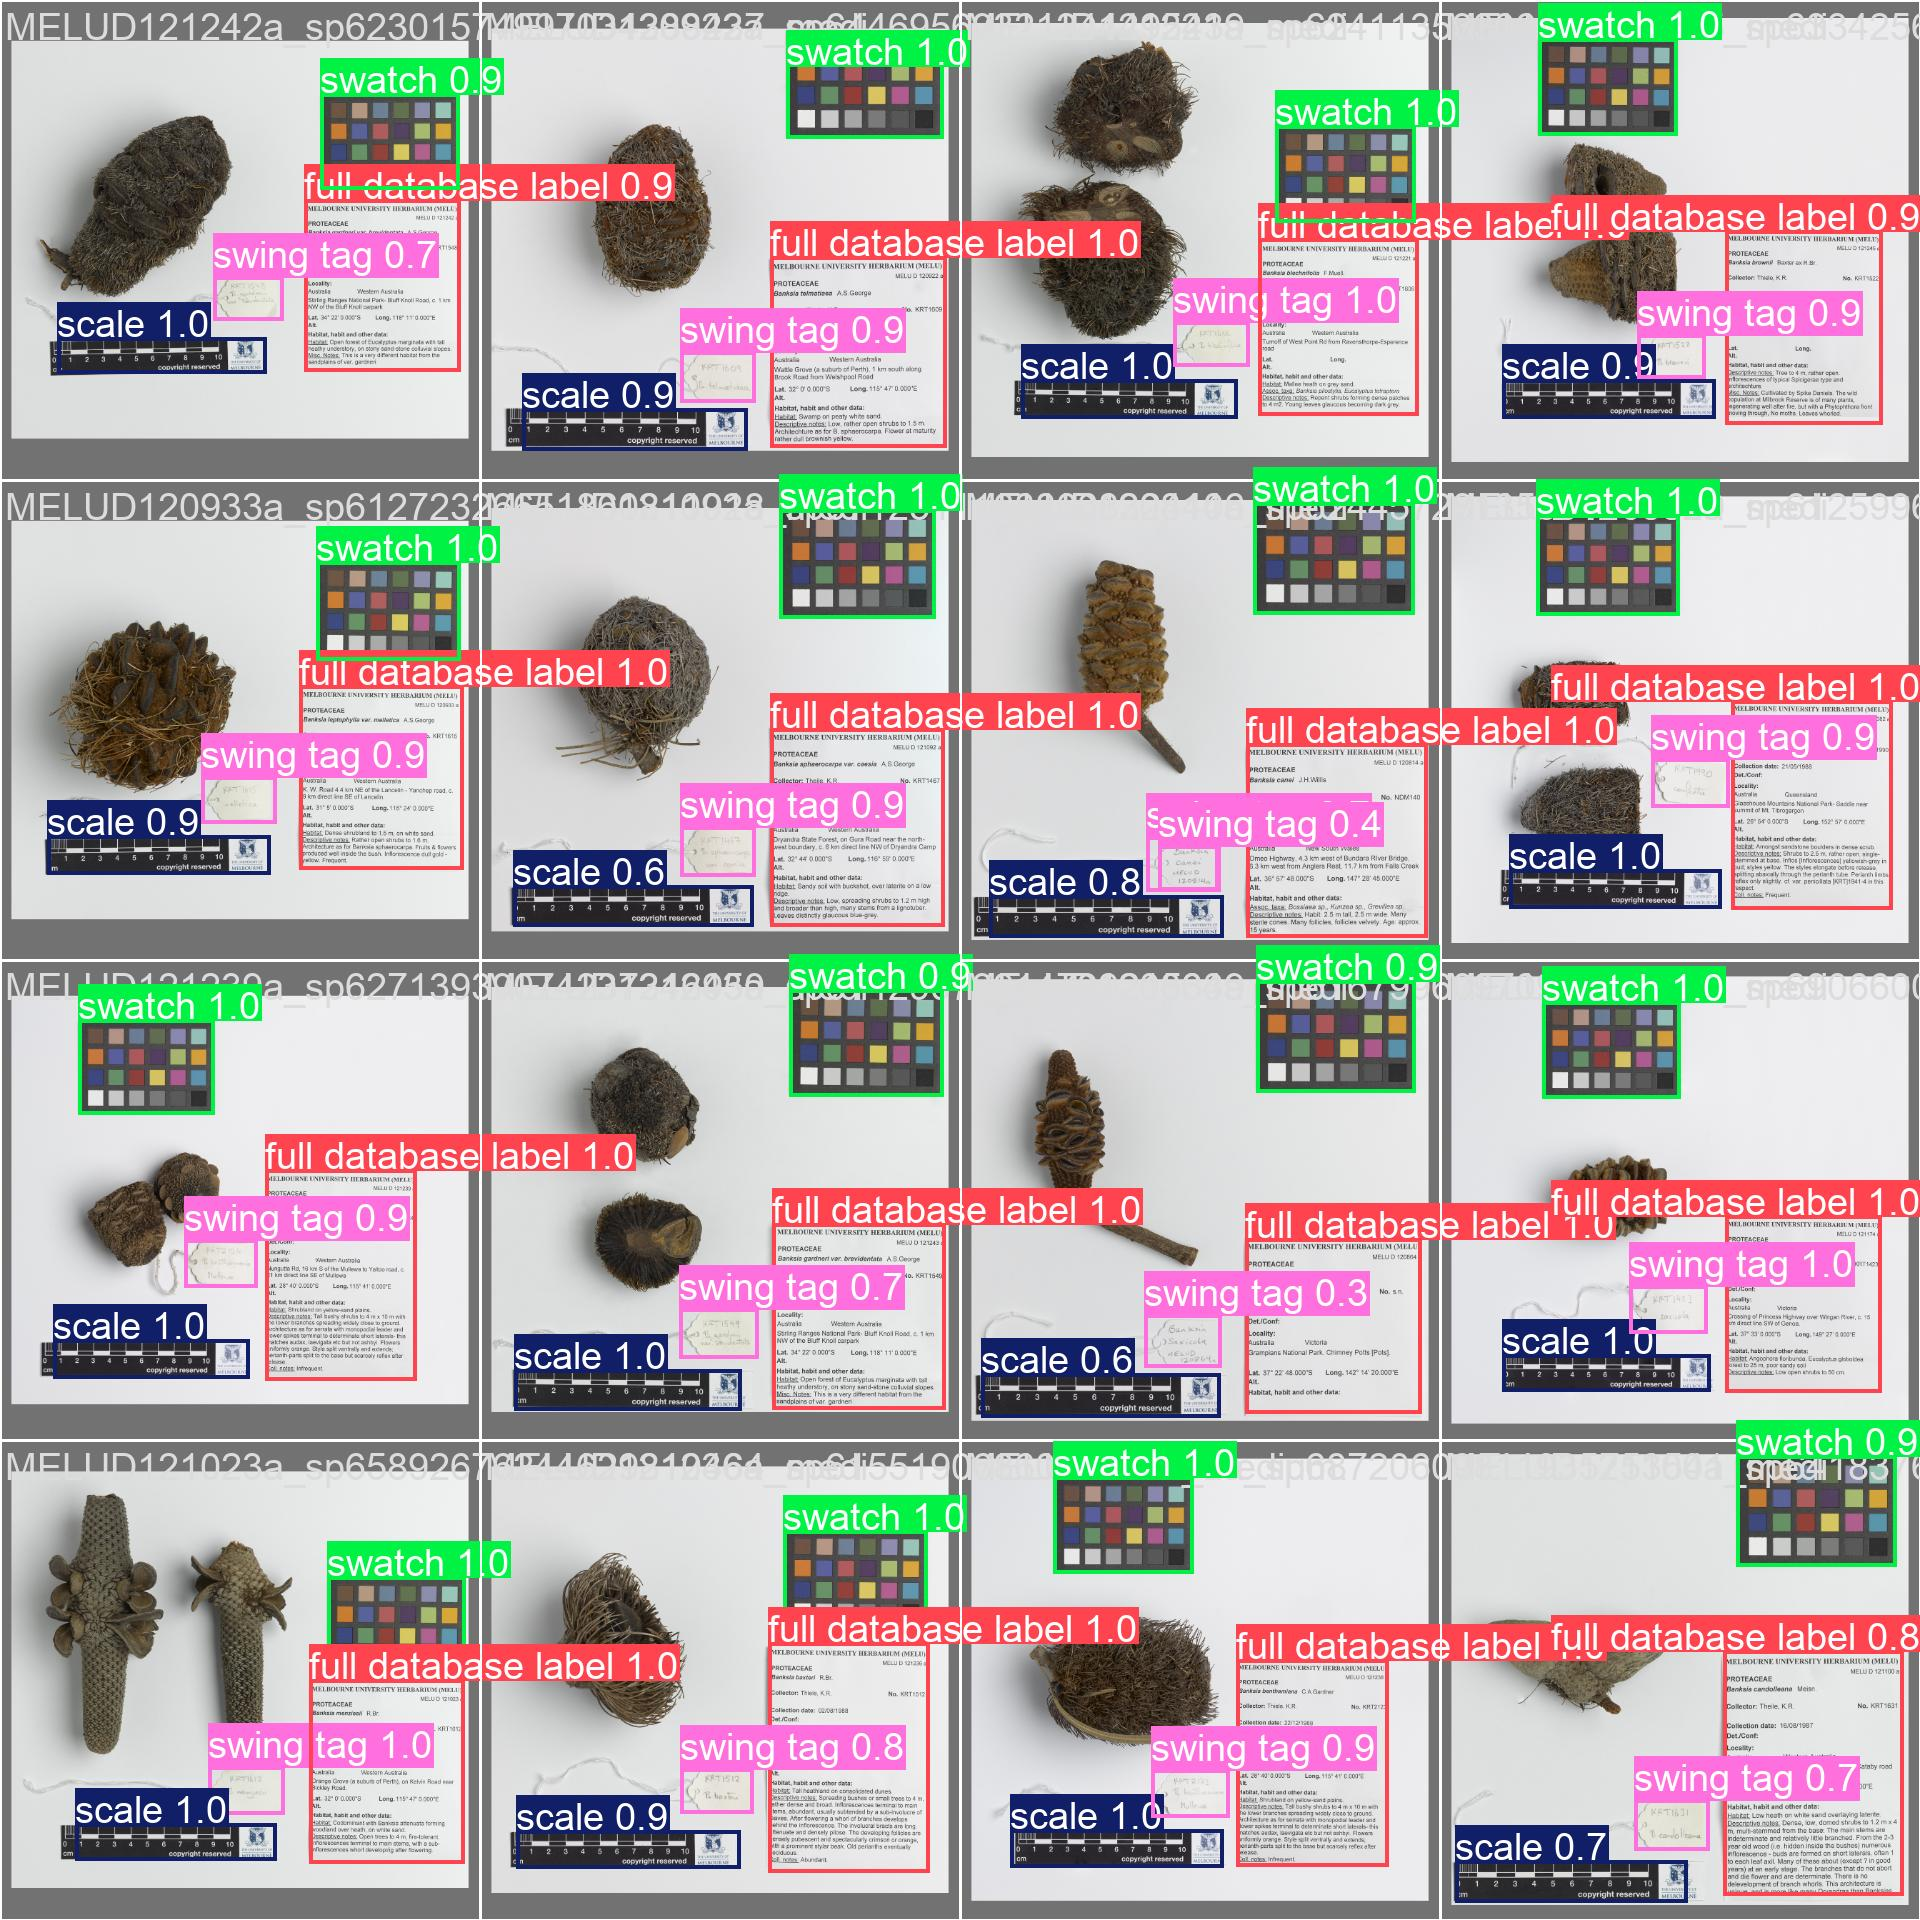
\includegraphics[width=\textwidth]{00Figuras/val_batch1_predMelu.jpg}
    \caption{Performance de modelo YOLO con datos MELU}
    \label{fig:image4}
  \end{subfigure}
  \vspace{0.5cm}
\end{figure}



\section{Primeras detecciones}

La primera etapa del proceso se enfocó en determinar el mejor modelo base para la
arquitectura federada, para ello se hizo uso de las matrices de confusión normalizadas
que en esencia brindan un panorama completo y robusto de cómo está funcionando la tarea
de clasificación para un modelo. A continuación se presentan las matrices asociadas a
los tres modelos considerados.
\begin{figure}[H]
  \centering
  \vspace{0.5cm}
  \begin{subfigure}[b]{0.48\textwidth}
    \includegraphics[width=\textwidth]{00Figuras/lone_confusion_matrix_unal.png}
    \caption{Performance de modelo YOLO con datos UN}
    \label{fig:image3}
  \end{subfigure}
  \hfill
  \begin{subfigure}[b]{0.48\textwidth}
    \includegraphics[width=\textwidth]{00Figuras/lone_confusion_matrix_melu.png}
    \caption{Performance de modelo YOLO con datos MELU}
    \label{fig:image4}
  \end{subfigure}
  \vspace{0.5cm}
\end{figure}

Ahora se presentan las matrices de confusión para el modelo fundacional (YOLO) aplicado las técnicas de aprendizaje federado, donde se evidencia una mejora marginal en la clasificación de artefactos respecto a los modelos individuales.

\begin{figure}[H]
  \centering
  \vspace{0.5cm}
  \begin{subfigure}[b]{0.48\textwidth}
    \includegraphics[width=\textwidth]{00Figuras/confusion_matrix_unal.png}
    \caption{Performance de modelo federado con datos UN}
    \label{fig:image3}
  \end{subfigure}
  \hfill
  \begin{subfigure}[b]{0.48\textwidth}
    \includegraphics[width=\textwidth]{00Figuras/confusion_matrix_melu.png}
    \caption{Performance de modelo federado con datos MELU}
    \label{fig:image4}
  \end{subfigure}
  \vspace{0.5cm}
\end{figure}

De estas se derivó la segunda etapa que fue la de construir una arquitectura federada
capaz de simular el proceso que un herbario debería hacer para poder usar esta
herramienta. A continuación se presentan los resultados del modelo fundacional (YOLO)
aplicado a los distintos sets de datos bajo la modalidad federada de aprendizaje
distribuido; en la siguiente sección se entrará en detalles de la significación de
estos gráficos.

\section{Modelo Federado}

\subsection{Precision Promedio Media (mAP@0.5)}

Presentamos primero un gráfico comparativo del rendimiento de las diferentes estrategias
de agregación, donde se evidencia una ganancia marginal respecto al método de agregación.

\begin{figure}[H]
  \centering
  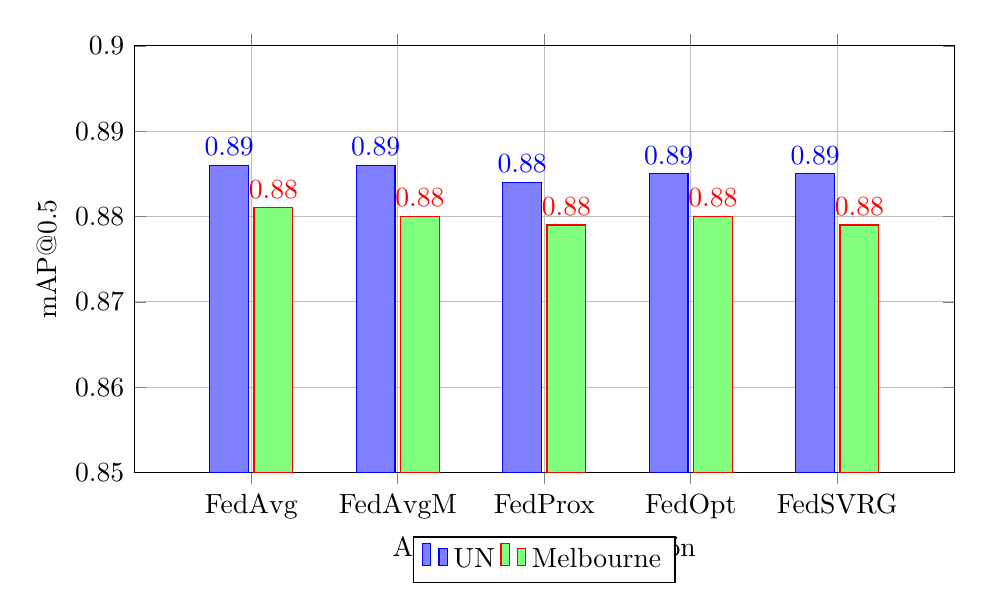
\begin{tikzpicture}
    \begin{axis}[
      ybar,
      bar width=14pt,
      width=12cm,
      height=7cm,
      ylabel={mAP@0.5},
      xlabel={Algoritmo de Agregación},
      symbolic x coords={FedAvg,FedAvgM,FedProx,FedOpt,FedSVRG},
      xtick=data,
      ymin=0.85, ymax=0.90,
      legend style={at={(0.5,-0.15)},anchor=north,legend columns=2},
      nodes near coords,
      nodes near coords align={vertical},
      enlarge x limits=0.2,
      grid=both
    ]
      \addplot+[fill=blue!50] coordinates {
        (FedAvg,0.886) (FedAvgM,0.886) (FedProx,0.884) (FedOpt,0.885) (FedSVRG,0.885)};
      \addplot+[fill=green!50] coordinates {
        (FedAvg,0.881) (FedAvgM,0.880) (FedProx,0.879) (FedOpt,0.880) (FedSVRG,0.879)};
      \legend{UN, Melbourne}
    \end{axis}
  \end{tikzpicture}
  \caption{Comparación de mAP@0.5 promedio por algoritmo de agregación y conjunto de datos.}
  \label{fig:map_bar}
\end{figure}

Las siguientes métricas se reportan con un \emph{umbral de confianza alto}, donde el
modelo opera en un régimen conservador minimizando falsos positivos.
$\mathrm{mAP}_{50}$ integra precision-recall sobre todas las clases:
\[
  \mathrm{mAP}_{50} = \frac{1}{C}\sum_{c=1}^{C}\int_0^1 p_c(r)\,dr
  \qquad\text{en } \mathrm{IoU} \ge 0.50
\]

\medskip
\begin{table}[H]
  \centering
  \caption{mAP$_{50}$ promedio por estrategia de agregación y conjunto de datos.}
  \small
  \begin{tabular}{lccr}
    \toprule
    \textbf{Algoritmo} & \textbf{UN} & \textbf{Melbourne} & $\Delta$ \textbf{(UN$-$Melb)} \\
    \midrule
    FedAvg  & 0.886 & 0.881 & $+$0.005 \\
    FedAvgM & 0.886 & 0.880 & $+$0.006 \\
    FedProx & 0.884 & 0.879 & $+$0.005 \\
    FedOpt  & 0.885 & 0.880 & $+$0.005 \\
    FedSVRG & 0.885 & 0.879 & $+$0.006 \\
    \midrule
    \textbf{Promedio} & \textbf{0.885} & \textbf{0.880} & $+$0.005 \\
    \bottomrule
  \end{tabular}
\end{table}

\medskip
\begin{table}[H]
  \centering
  \caption{Precision promedio con umbral de confianza alto $\hat{p}_o \ge s_{\text{conf}}^{\text{high}}$.}
  \small
  \begin{tabular}{lccr}
    \toprule
    \textbf{Algoritmo} & \textbf{UN} & \textbf{Melbourne} & $\Delta$ \textbf{(UN$-$Melb)} \\
    \midrule
    FedAvg  & 0.97 & 0.96 & $+$0.01 \\
    FedAvgM & 0.97 & 0.96 & $+$0.01 \\
    FedProx & 0.96 & 0.95 & $+$0.01 \\
    FedOpt  & 0.97 & 0.96 & $+$0.01 \\
    FedSVRG & 0.96 & 0.95 & $+$0.01 \\
    \midrule
    \textbf{Promedio} & \textbf{0.966} & \textbf{0.956} & $+$0.010 \\
    \bottomrule
  \end{tabular}
\end{table}

El Recall se evalúa con un \emph{umbral de confianza bajo}, donde el modelo maximiza
la recuperación de verdaderos positivos al costo de más falsos positivos.
El F1-score balancea ambos regímenes:
\[
  \mathrm{Recall} = \frac{\mathrm{VP}}{\mathrm{VP}+\mathrm{FN}},\qquad
  \mathrm{Precision} = \frac{\mathrm{VP}}{\mathrm{VP}+\mathrm{FP}},\qquad
  F_1 = \frac{2\cdot\mathrm{Precision}\cdot\mathrm{Recall}}{\mathrm{Precision}+\mathrm{Recall}}
\]

\medskip
\begin{table}[H]
  \centering
  \caption{Recall promedio con umbral de confianza bajo $\hat{p}_o \ge s_{\text{conf}}^{\text{low}}$.}
  \small
  \begin{tabular}{lccr}
    \toprule
    \textbf{Algoritmo} & \textbf{UN} & \textbf{Melbourne} & $\Delta$ \textbf{(UN$-$Melb)} \\
    \midrule
    FedAvg  & 0.99 & 0.98 & $+$0.01 \\
    FedAvgM & 0.99 & 0.98 & $+$0.01 \\
    FedProx & 0.98 & 0.98 & $\phantom{+}$0.00 \\
    FedOpt  & 0.99 & 0.98 & $+$0.01 \\
    FedSVRG & 0.98 & 0.97 & $+$0.01 \\
    \midrule
    \textbf{Promedio} & \textbf{0.986} & \textbf{0.978} & $+$0.008 \\
    \bottomrule
  \end{tabular}
\end{table}

\begin{table}[H]
  \centering
  \caption{Máxima puntuación $F_1$ promedio por estrategia de agregación y conjunto de datos.}
  \small
  \begin{tabular}{lccr}
    \toprule
    \textbf{Algoritmo} & \textbf{UN} & \textbf{Melbourne} & $\Delta$ \textbf{(UN$-$Melb)} \\
    \midrule
    FedAvg  & 0.85 & 0.84 & $+$0.01 \\
    FedAvgM & 0.85 & 0.84 & $+$0.01 \\
    FedProx & 0.84 & 0.83 & $+$0.01 \\
    FedOpt  & 0.85 & 0.84 & $+$0.01 \\
    FedSVRG & 0.84 & 0.83 & $+$0.01 \\
    \midrule
    \textbf{Promedio} & \textbf{0.846} & \textbf{0.836} & $+$0.010 \\
    \bottomrule
  \end{tabular}
\end{table}

La brecha consistente $\Delta \in [0.000,\,0.010]$ en todas las métricas y todas
las estrategias confirma que el origen del conjunto de datos (UN vs.\ Melbourne) es una
fuente de varianza mayor que la elección del algoritmo de agregación.